% The packages used here are just a sample. You may need others, and may not need some of these. It doesn't hurt to leave them in, unless they start to conflict with other packages you've added. Chapter 2 has example code for equations, figures, tables, citations, abbreviations, etc. If there are sections labeled 'optional' that you don't want, just comment them out. -jg
\documentclass[reqno,12pt,oneside]{report} % right-side equation numbering, 12 point font, print one-sided 
%\documentclass[reqno,12pt,twoside,openright]{report} % right-side equation numbering, 12 point font, print two-sided, Chapters start on odd pages. Rackham only accepts one-sided, so this is for personal printings.

\usepackage{rac}         % Use Rackham thesis style file
\usepackage{aas_macros}  % To allow the reading of ADS journal references in the bibliography
\usepackage[intlimits]{amsmath} % Puts the limits of integrals on top and bottom
\usepackage{amsxtra}     % Use various AMS packages
\usepackage{amsthm}
\usepackage{amssymb}
\usepackage{amsfonts}
\usepackage{graphicx}    % Add some packages for figures. Read epslatex.pdf on ctan.tug.org
\usepackage{rotating}
\usepackage{color}
\usepackage{epsfig}
\usepackage{subcaption}   % To make subfigures. Read subfigure.pdf on ctan.tug.org
\usepackage{float}
%\usepackage{subcaption}
\usepackage{verbatim}
\usepackage[hidelinks]{hyperref}
\usepackage[numbers]{natbib}      % Allows you to use BibTeX
\usepackage[printonlyused]{acronym} % For the List of Abbreviations. Read acronym.pdf on ctan.tug.org
\usepackage{setspace}    % Allows you to specify the line spacing
\usepackage{multirow}
\usepackage{caption}
\usepackage{bm}
\usepackage{xfrac}
\usepackage{enumitem}

\captionsetup[figure]{textfont=small}
\captionsetup[subfigure]{labelfont=bf,textfont=scriptsize ,singlelinecheck=false, justification=raggedright}
\renewcommand\arraystretch{1.2}

%\usepackage{geometry}
\onehalfspacing         % \onehalfspacing for 1.5 spacing, \doublespacing for 2.0 spacing.
\newcommand{\sun}{\ensuremath{\odot}} % sun symbol is \sun
\newcommand{\metrel}{$E_{\text T}^{\text {miss,rel}}$}
\newcommand{\dileptonmass}{$m_{\ell \ell}$}
\newcommand{\mttwo}{$m_{\text{T2}}$}
\newcommand{\invfb}{fb\textsuperscript{-1}}
\newcommand{\lumi}{$\int \mathcal{L} \, \mathrm{dt}$}
%%%%%%%%%%%%%%%%%%%%%%%%%%%%%%%%%%%%%%%%%%%%%%%%%%%%%%%%%%%%%%%%%%%%%%%%%%%%%%%

% Various theorem environments. All of the following have the same numbering
% system as theorem.

\theoremstyle{plain}
\newtheorem{theorem}{Theorem}
\newtheorem{prop}[theorem]{Proposition}
\newtheorem{corollary}[theorem]{Corollary}
\newtheorem{lemma}[theorem]{Lemma}
\newtheorem{question}[theorem]{Question}
\newtheorem{conjecture}[theorem]{Conjecture}
\newtheorem{assumption}[theorem]{Assumption}

\theoremstyle{definition}
\newtheorem{definition}[theorem]{Definition}
\newtheorem{notation}[theorem]{Notation}
\newtheorem{condition}[theorem]{Condition}
\newtheorem{example}[theorem]{Example}
\newtheorem{introduction}[theorem]{Introduction}

\theoremstyle{remark}
\newtheorem{remark}[theorem]{Remark}


%%%%%%%%%%%%%%%%%%%%%%%%%%%%%%%%%%%%%%%%%%%%%%%%%%%%%%%%%%%%%%%%%%%%%%%%%%%%%%%

\numberwithin{theorem}{chapter}     % Numbers theorems "x.y" where x
                                    % is the section number, y is the
                                    % theorem number

%\renewcommand{\thetheorem}{\arabic{chapter}.\arabic{theorem}}

%\makeatletter                      % This sequence of commands will
%\let\c@equation\c@theorem          % incorporate equation numbering
%\makeatother                       % into the theorem numbering scheme

%\renewcommand{\theenumi}{(\roman{enumi})}

%%%%%%%%%%%%%%%%%%%%%%%%%%%%%%%%%%%%%%%%%%%%%%%%%%%%%%%%%%%%%%%%%%%%%%%%%%%%%%

% If printing two-sided, this makes sure that any blank page at the 
% end of a chapter will not have a page number. 
\makeatletter
\def\cleardoublepage{\clearpage\if@twoside \ifodd\c@page\else
\hbox{}
\thispagestyle{empty}
\newpage
\if@twocolumn\hbox{}\newpage\fi\fi\fi}
\makeatother 

%%%%%%%%%%%%%%%%%%%%%%%%%%%%%%%%%%%%%%%%%%%%%%%%%%%%%%%%%%%%%%%%%%%%%%%%%%%%%%

%This command creates a box marked ``To Do'' around text.
%To use type \todo{  insert text here  }.

\newcommand{\todo}[1]{\vspace{5 mm}\par \noindent
\marginpar{\textsc{To Do}}
\framebox{\begin{minipage}[c]{0.95 \textwidth}
\tt\begin{center} #1 \end{center}\end{minipage}}\vspace{5 mm}\par}

%%%%%%%%%%%%%%%%%%%%%%%%%%%%%%%%%%%%%%%%%%%%%%%%%%%%%%%%%%%%%%%%%%%%%%%%%%%%%%%
\begin{document}

\bibliographystyle{ieeetr}    % Set the bibliography style. agu04, plain, alpha, etc.

% Title page as required by Rackham dissertation guidelines
\titlepage{Sensitivity studies for searches for electroweak supersymmetry during run-II of the LHC}{Sesegma Sanzhieva}{Bachelor of Science}
{Atmospheric and Space Sciences}{2008}
{}

% Begin the front matter as required by Rackham dissertation guidelines
\initializefrontsections

% Optional Frontispiece
%\frontispiece{
\includegraphics[width=6in]{Intro/Happy} Find a cool picture to go here.}

% Optional, but recommended, Copyright page
%\copyrightpage{Your Name}

% Page numbering. If you don't include a frontispiece or copyright page, you'll need to change this for two-sided printing.
\makeatletter
\if@twoside \setcounter{page}{4} \else \setcounter{page}{1} \fi
\makeatother
 
% Optional Dedication page
%\dedicationpage{For all the people}

% Optional Acknowledgements page
%\startacknowledgementspage
%Thanks to the people who made this dissertation possible, especially those who put together a nice \LaTeX\, template for me to use.
%\label{Acknowledgements}

% Optional Preface page
%\startprefacepage
%\input{Preface}
%\label{Preface}

% Table of contents, list of figures, etc.
\tableofcontents     % Required
%\listoffigures       % Required if there is more than one figure
%\listoftables        % Required if there is more than one table
%\listofmaps          % Required if there is more than one map
%\listofappendices    % Required if there is more than one appendix
%\listofabbreviations % Optional. Abbreviations should be stored in a file named abbr.tex

% Optional in-dissertation Abstract Page
\startabstractpage
{Sensitivity studies for searches for electroweak supersymmetry during run-II of the LHC}{Sesegma Sanzhieva}{}


\label{Abstract}

\startthechapters
% The individual files for each of the chapters are put here.
% Save each chapter of your thesis to a seperate tex file
% and then use the \input command to include this file in your
% thesis.  For instance you can save a file to "intro.tex" and 
% then type \input{intro}. 

 \chapter{Introduction}
 \label{chap:Intro}
 High Energy Physics (HEP) is a branch of physics that studies elementary particles. The main way of studying physics experimentally at subatomic level is using particle accelerators. Specific particles are accelerated to high speeds and directed to collide with each other producing an array of other particles that are then registered by detectors and studied by physicists. The largest currently functioning HEP experiment is the Large Hadron Collider (LHC) at CERN in Geneva, Switzerland. Since 2015, it is able to accelerate protons and create collisions at a centre-of-mass energy of 13 TeV. These collisions happen at two sites where the main particle detectors are situated. These experiments are ATLAS (A Toroidal LHC Apparatus) and CMS (Compact Muon Solenoid). Such high energy conditions of collisions emulate the state of the universe very shortly after the Big Bang and thus allow creation of particles that don't exist at normal conditions. 

The underlying theory of modern HEP is the Standard Model (SM) and it has been very successful in describing subatomic particles and the interactions between them. It is a very robust theory that has been tested through a plethora of experiments at colliders. The most prominent success of previous LHC runs at 7 and 8 TeV centre-of-mass energy was the discovery of the Higgs particle, which 
was the final SM particle whose existence was proven experimentally \citep{Aad:2012tfa,chatrchyan2012observation}.   

However, there are limitations to SM and there are a number of theories that try address these shortcomings. Collectively they are known as “Beyond-the-Standard-Model” (BSM) theories and present new theoretical frameworks aiming to explain physical world at a deeper level. One of the major BSM theories is supersymmetry (SUSY). It has a mathematically effective and elegant representation and, most importantly, overcomes some critical SM limitations.

Searches for evidence of supersymmetry are performed at the LHC along with other particle experiments. After runs at 7 and 8 TeV no significant evidence was found and limits on masses of hypothetical supersymmetric particles have been placed. Higher energy collisions present a better chance of finding  evidence of supersymmetry. The research presented in this thesis focuses on trying to design search methods in run-II (13 TeV) data that are sensitive to particular SUSY scenarios that feature electroweak production and decay. For that purpose a set of kinematic and topological variables are investigated as ways to determine presence of new particles.


 \chapter{Background information}
 \label{chap:bg}
 \section{The Standard Model}
\label{SM}
\subsection{The overview of the Standard Model}
The underlying theory of modern High Energy Physics is the Standard Model (SM). This theory has been developed in the second half of the 20th century with contributions from many scientists and it is a very successful representation of the world on the subatomic level.
The SM classifies all known subatomic particles into specific categories and provides the description of the interactions between them. 

In the SM there are two main types of fermions (1/2-spin particles) known as quarks and leptons. Each family has three generations with each consecutive generation being heavier than the previous. The up and down quarks along with the electron are stable and constitute ordinary matter. The interactions between fermions are mediated through the exchange of force carrier particles known as gauge bosons (see Tab.~\ref{tab:SM}). The final piece in the SM is the Higgs boson and it gives mass to other fundamental particles. All bosons possess integer spin \citep{martin2006nuclear}. Further nomenclature identifies hadrons - composite particles that are made of quarks and gluons. 
\begin{table}[]
\centering
\label{my-label}
\begin{tabular}{cccc | ll}
\textbf{Fermion}                  & \multicolumn{3}{c}{\textbf{Generations}} & \multicolumn{2}{c}{\textbf{Bosons}} \\ \hline
\multirow{2}{*}{\textbf{Leptons}} & $e$        & $\mu$        & $\tau$       & $Z$            & Higgs           \\
                                  & $\nu_{e}$  & $\nu_{\mu}$  & $\nu_{\tau}$ & $W^{\pm}$            &                 \\ 
\multirow{2}{*}{\textbf{Quarks}}  & $u$        & $c$          & $t$          & photon            &                 \\
                                  & $d$        & $s$          & $b$          & gluon             &          \\ \hline      
\end{tabular}
\caption{The Standard Model particles}
\label{tab:SM}
\end{table}

The mathematical representation of the SM is built within the broader frame of Group Theory. Employing the official terminology, the SM has the symmetry group U(1)$_{\text{Y}}\times$SU(2)$_{\text{L}}\times$SU(3). The SU(3) symmetry group generates strong interactions, that describe processes involving quarks and gluons. These processes are described by the theory of Quantum Chromodynamics and the particles possess a specific type of charge known as ``colour charge".
The U(1)$_{\text{Y}}\times$SU(2)$_{\text{L}}$ group generates electroweak interactions. At energies below 100 GeV, however, the single electroweak interaction is broken into the weak and electromagnetic varieties with the symmetry group U(1)$_{\text{em}}$. 
The unification of these two types was the result of efforts by Glashow, Weinberg and Salam \citep{Glashow:1961tr,weinberg1967model,salam1968elementary}. 
The weak interaction processes involve fermions and are mediated by electrically charged W\textsuperscript{$\pm$} bosons for charged processes and the chargeless Z gauge boson for neutral ones. Finally, the electromagnetic force is mediated by photons and only involves electrically charged particles. 

Above the unification energy of 100 GeV, and thus before the spontaneous electroweak symmetry breaking  through Higgs mechanism \citep{englert1964broken, higgs1964broken}, the gauge bosons are different. There are three W bosons, denoted W\textsuperscript{1}, W\textsuperscript{2}, W\textsuperscript{3} corresponding to the SU(2)$_{\text{L}}$ part of the group and one B boson corresponding to the U(1)$_{\text{Y}}$ part. 
All the electroweak bosons are massless, and acquire mass by coupling to the Higgs field in the process of symmetry breaking.  

\subsection{Limitations of the SM}

The predictions of the SM have been successfully tested in particle accelerator experiments, and its final confirmation came with the discovery of the Higgs boson in 2012 - a true scientific breakthrough. This was the last missing piece of experimental evidence needed for the full validation of the SM. The experiments that led to this discovery were conducted at CERN’s Large Hadron Collider (LHC) in run-I proton-proton collisions at centre-of-mass energy $\sqrt{s}=$7 and the later upgrade to 8 TeV.  
Despite the fact that the SM has proven to be an extremely precise and successful theory there are some caveats for which it does not provide  adequate solutions. 

One of the inconsistencies within the SM is the so-called Hierarchy problem \citep{PhysRevD.14.1667}. One of the ways it reveals itself is through the large discrepancy between the Planck mass and the mass of the Higgs particle. The former is about $10^{17}$ times bigger than the latter and current representation of particle physics cannot explain such a big difference. Quantum effects start manifesting themselves at the Plank mass threshold and such a vast difference between these two values is yet unaccounted for. 

Another prominent problem is that the SM does not explain dark matter. While ordinary matter only constitutes about 5\% in the total mass-energy content of the universe, it is dark matter and dark energy that account for the rest \citep{ade2014planck}. 
%However,
The SM does not provide a candidate particle for dark matter and thus is only able to describe ordinary matter and energy. 

One of the main challenges of modern physics is the unification of forces. This is part of the ongoing attempts to reach the ultimate goal - a ``theory of everything". Such a theory would have to account for all physical aspects of the universe and include the most fundamental structures and interactions. The first step was made with the unification of electromagnetic and weak forces.  
The next step is to achieve the unification of electromagnetic, weak, and strong interaction forces – this step is the Grand Unification. The ultimate step is to combine all four fundamental forces together, which means adding gravity, in what is called Super Unification (see Fig.~\ref{fig:unification}). Thus far quantum field theory and general relativity are able to describe phenomena on their respective scale of action with remarkable precision, but are fundamentally incompatible.  
\begin{figure}[ht]
		\centering
			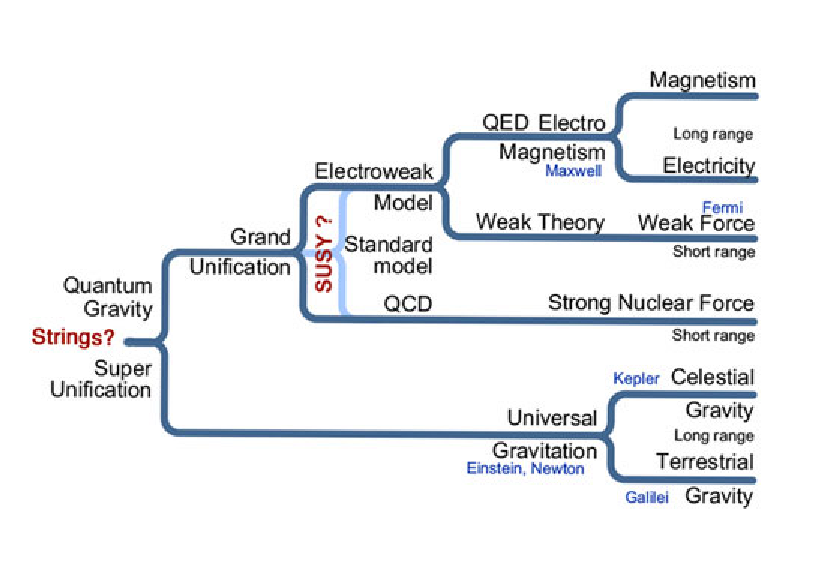
\includegraphics[scale=0.8]{Chap2/Unification}
\caption[Unification of forces]{\label{fig:unification} Various stages in the unification of forces  \citep{unification}}.
\end{figure}

Within the confines of the SM even the Grand Unification is not possible, and this prompts the search for new theories that account for this and other shortcomings of the SM. Collectively they are called Beyond-Standard-Model (BSM) theories. Among these, there are theories that include extra-dimensions, composite Higgs boson models, etc. Theoretical and experimental search for BSM physics is the current frontier of HEP and one of the most important questions in science overall. 


\section{Supersymmetry}
One of the strongest candidate framework theories that can offer solutions to the SM deficiencies is supersymmetry (SUSY) \citep{Lykken:1996xt}. SUSY is a spacetime symmetry that equates fermionic and bosonic degrees of freedom. Among several theories that are based on SUSY principles, the Minimal Supersymmetric Standard Model (MSSM) offers the simplest extention of the SM. The MSSM postulates that each SM particle has a supersymmetric partner which is  different only in spin by one-half unit %(see Table~\ref{tab:MSSMparticles}), 
while all other quantum numbers stay the same. 
%\vspace{0.5cm}
%\begin{table}
%\captionsetup{width=0.8\textwidth}
%\def\arraystretch{1.5}
%\centering
%\begin{tabular}{|l|c| l|}
%\hline 
%name & spin & particles \\ 
%\hline 
%squarks & 0 & $\tilde{d}_{L},\tilde{u}_{L},\tilde{s}_{L},\tilde{c}_{L}, \tilde{b}_{1}, \tilde{t}_{1}, \tilde{d}_R,\tilde{u}_{R},\tilde{s}_{R},\tilde{c}_{R},\tilde{b}_{2}, \tilde{t}_{2} $\\ 
%sleptons & 0 & $\tilde{e}_L, \tilde{\nu}_{eL}, \tilde{\mu}_L, \tilde{\nu}_{\mu L}, \tilde{\tau}_1, \tilde{\nu}_{\tau L}, \tilde{e}_R,\tilde{\mu}_R, \tilde{\tau}_2 $\\ 
%charginos & $1/2$ & $\tilde{\chi}_1^{\pm} ,\, \tilde{\chi}_2^{\pm}  $ \\ 
%neutralinos & $1/2$ & $\tilde{\chi}_1^{0},\, \tilde{\chi}_2^{0},\,\tilde{\chi}_3^{0},\, \tilde{\chi}_4^{0} $\\ 
%gluino & $1/2$ & $\tilde{g}$ \\  
%Higgs & 0 & $h^{0},\, H^{0},\, A^{0},\, H^{\pm}$ \\ 
%\hline 
%\end{tabular} 
%\caption{\label{tab:MSSMparticles} SUSY particles in the MSSM where subscript $R$ denotes right-handed particles and $L$ - left-handed ones. $H^0$ Higgs boson also exists in the SM. }
%\end{table}
The superpartners of quarks, leptons, and neutrinos are called squarks, sleptons and sneutrinos. For gauge bosons the superpartners are  gluinos, photino, winos and binos, collectively named gauginos. The latter two are superpartners of the  B and three W bosons of the elecroweak interaction before electroweak symmetry breaking. It follows naturally since SUSY is invoked before the electroweak symmetry breaking. The Higgs sector in SUSY has five superpartners  - two charged $(H^{\pm})$ sparticles and three neutral ones $(h^0, H^0, A^0)$. They are known collectively as Higgsinos. Mixing between winos, binos and Higgsinos results in charginos and neutralinos. Their mass eigenstates are referred to as $\tilde{\chi}^{\pm}_{i}$ ($i$ = 1,2) and $\tilde{\chi}^{0}_{i}$ ($i$ = 1,2,3,4) in order fo increasing mass. 

The MSSM belongs to a class of theories that all share the same requirement - a quantity known as R-parity has to be conserved in interactions. The mathematical description of R-parity is beyond the scope of this paper. However, one important consequence of R-parity conservation is that if supersymmetric particles were to be produced in collisions, they will be created in pairs. Then they decay through various possible scenarios with the lightest supersymmetric particle (LSP) emerging in the final state and escaping undetected. Because the LSP is stable it provides a possible candidate for the dark matter particle.

The MSSM imposes 105 free parameters and this is one of its major issues, since any analysis will be addled with enormous complexity stemming from high dimensionality. There are various simplified models that reduce the number of free parameters to manageable values through various theoretically and experimentally motivated constraints. One of them is the phenomenological Minimal Supersymmetric Standard Model (pMSSM) that contains only 19 free parameters and which will be used in this thesis' analysis. 





\section{The ATLAS detector}
\label{sec:atlas}
The ATLAS experiment is a multi-purpose particle detector with cylindrical geometry and has a nominal forward-backward symmetry \citep{aad2008atlas}. The dimensions of the detector are 25 m in height and 44 m in length and the overall weight of the detector is approximately 7000 tonnes.
It can detect particles with almost 4$\pi$ coverage in solid angle around the collision point, which covers almost all of the spherical area around the center. 

Proton bunches are accelerated in the underground ring that is 27 km in diameter and are directed to collide inside the detectors. The collisions happen at 40 MHz bunch crossing rate, with an average 23 interactions per bunch crossing. The LHC is designed to operate at $\sqrt{s}$=14 TeV and instantaneous luminosity $\mathcal{L} = 10^{34}$ cm\textsuperscript{-2} s\textsuperscript{-1} in proton-proton collision mode. Instantaneous luminosity is defined as follows
\begin{equation}
\mathcal{L} = \frac{1}{\sigma}\frac{dN}{dt}
\end{equation}  
Where $\sigma$ is the interaction cross-section, and $N$ is the number of detected events during time $t$. Integrated luminosity $\int \mathcal{L}\, dt$ is a quantity that expresses the amount of total data gathered during the time $t$ of running the LHC. Luminosity  is particularly useful as a way to express the amount of data gathered, because it allows to find number of events for a particular process simply by multiplying this process's cross-section by the value of luminosity. The analysis presented in this paper uses the dataset recorded at 3.2 fb\textsuperscript{-1} of integrated luminosity throughout run-II of the LHC during 2015. 

%Add something about cross sections!!!!!!

\begin{figure}[!t]
	\centering
    \captionsetup{width=\textwidth}
	\includegraphics[width=\textwidth]{Chap2/ATLAS_SE_WithDimensions_Corrected.png}
\caption[Cut-away view of the ATLAS detector]{\label{fig:detector}  Cut-away view of the ATLAS detector (people are included for scale comparison) \citep{aad2008atlas}. }
\end{figure}

The Cartesian coordinate system used at ATLAS has its origin at the nominal point of interaction with the $z$ axis extending along the particle beam longitudinally, the positive $x$ axis pointing towards the center of the ring, and the positive $y$ axis pointing upwards. 
The geometry of the detector makes the use of cylindrical coordinate system especially convenient. Using it, the $z$ axis stays the same, the polar angle $\theta$ is the angle from the $z$-axis, and the azimuthal angle $\phi$ encircles the $z$ axis in the transverse plane. However, instead of $\theta$ it is more convenient to use pseudorapidity $\eta$, due to the fact that differences in pseudorapidity are close to invariant under Lorentz boosts along the $z$ axis (fully invariant for real rapidity). $\eta$ is defined as follows
\begin{equation}
\eta = -\ln\biggl(\tan\frac{\theta}{2}\biggr)
\end{equation}


\subsection{ The ATLAS sub-detectors and trigger systems}

The ATLAS detector consists of several subdetector layers with each layer performing a specific function (see Fig.~\ref{fig:event}). The Inner Detector (ID) performs tracking of newly created particles. It is closest to the collision point and covers $|\eta|<2.5$ in pseudorapidity. The ID has high granularity as it is exposed to the highest density of particle interaction. It was designed to provide a transverse momentum resolution and a transverse impact parameter resolution \citep{aad2010atlas}. The detector itself consists of three separate subsystems. The main components of the ID are the silicon pixel detector, the semiconductor tracker, and the transition radiation tracker. Ahead of the run-II a new pixel layer, called the Insertable B-Layer (IBL), has been added to the ID improving the resolution and particle identification qualities. All these layers are immersed in a 2 T magnetic field, created by the thin superconducting solenoidal magnet. This field is parallel to the beam axis and bends trajectories of charged particles allowing their charge and momentum identification based on the characteristic bending of their trajectories. 
\begin{figure}[!h]
	\centering
    \captionsetup{width=0.9\textwidth}
	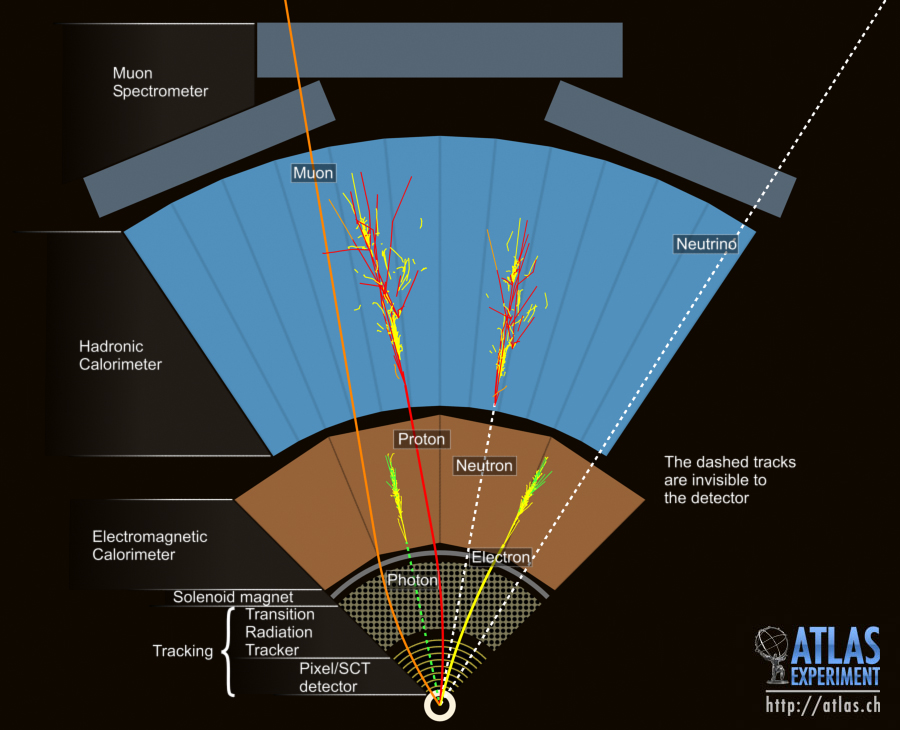
\includegraphics[width=0.9\textwidth]{Chap2/0803022_01.jpg}
\caption[Event in the transverse plane]{\label{fig:event} Event in the transverse plane, a computer generated image of the ATLAS detector \cite{event}. }
\end{figure}

The next two layers are the two calorimeters that measure energies of specific types of particles. The particles travel through the detectors and lose their energy via interaction with its layers leaving energy deposits as they move through the material. 
The first one is the high-granularity Electromagnetic Calorimeter (EmCal) and it measures energies of electrons and photons. Coloured particles (gluons and quarks) form ``jets" that travel further into Hadronic calorimeter (HCal) where they continue their decays and also deposit their available energy.
Both calorimeters are  designed to provide good quality measurements of momentum and energy and cover the region $|\eta|<4.9$.

The final detecting layer is the Muon spectrometer (MS), which tracks and measures charged particles, specifically muons. Muons do not interact with matter as strongly as electrons so they travel further without radiating much energy in the calorimeters.
MS is immersed into a large toroidal magnet, that provides a magnetic field throughout the spectrometer and bends the trajectories of charged muons, which makes it possible to detect their charge and momentum. Any particles that are not covered by the described sub-detectors will escape undetected. These include neutrinos and, possibly, the LSP. 

Triggers are used to select events by identifying signatures of various particles as well as using global event signatures, such as missing transverse energy \citep{aad2012performance}. A multilevel trigger system is used at ATLAS to select events that are of interest to further offline analysis. 
The  first  level is hardware-based and uses information from the calorimeters and muon spectrometer, the second and third levels are software-based and use information from all sub-detectors. Because the data at the LHC is produced in staggering amounts employing efficient trigger systems is crucial to be able to extract information that is relevant for further analysis. At $\sqrt{s}$=13 TeV the spacing between bunches crossing is 25 ns and the collision rate is 40 MHz. This rate has to be reduced to O(500 Hz) to be able to keep data in permanent memory devices \citep{barr2015particle}.

Ideally, a trigger should be able to retain a maximum number of events that are interesting for physics analysis and reject as many background events as possible. In this regard the concept of trigger efficiency is very important, and this efficiency varies depending on the particular process that is being investigated. The overall goal is to reduce data from the raw amount to the size at which it can be stored permanently and at the same time keeping  as many relevant events as possible. 

 
 \chapter{Search for supersymmetry at the LHC}
 \label{chap:searches}
\section{Introduction}

Searches for various BSM theories including SUSY have been performed at LHC  alongside searching for the Higgs and performing different SM anlyses. Many SUSY searches were conducted targeting the production of squarks and gluinos. This was motivated by a larger theoretical cross-section and therefore higher probability of producing coloured superpartners \cite{borschensky2014squark}. Up to this moment no statistically significant excess over SM has been detected and exclusion limits were placed on masses of SUSY particles. Figure~\ref{fig:SUSYlimit} shows the latest data on the masses that have been excluded for supersymmetric particles in various production scenarios. The lower limits on the masses of most squarks and gluinos in different searches significantly exceed 1 TeV \citep{aad2015summary}. As a consequence, if their production occurs, it is either extremely rare at present energies or requires higher energy of collision to leave an identifiable signature. 

This thesis's research will focus on the electroweak production as one of the possible SUSY particle production scenario. Sleptons and gauginos are produced in electroweak production processes and are not affected by the strong force. They have smaller cross-sections compared to squarks and gluinos, so their theoretical production rate is smaller. However, if their masses are small compared to the strongly interacting sparticles, SUSY production will likely be dominated by electroweak production where sparticles have smaller mass and current energy might be enough to produce them in quantities that would allow their detection \citep{aad2016search}.
%\newgeometry{left=1cm,right=1cm}
\begin{figure}[!ht]
\includegraphics[width=\textwidth]{Chap3/ATLAS_SUSY_Summary.png}
\caption{Exclusion limits of ATLAS searches for Supersymmetry \citep{SUSYlimits}}
\label{fig:SUSYlimit}
\end{figure}
\cleardoublepage


So far searches in the electroweak region have been unable to find evidence of supersymmetric particles. Limits on their masses according to various decay scenarios have been obtained and can be seen in Fig \ref{fig:summaryplot}.
\begin{figure}[!ht]
	\centering
	\captionsetup{width=0.8\textwidth}
	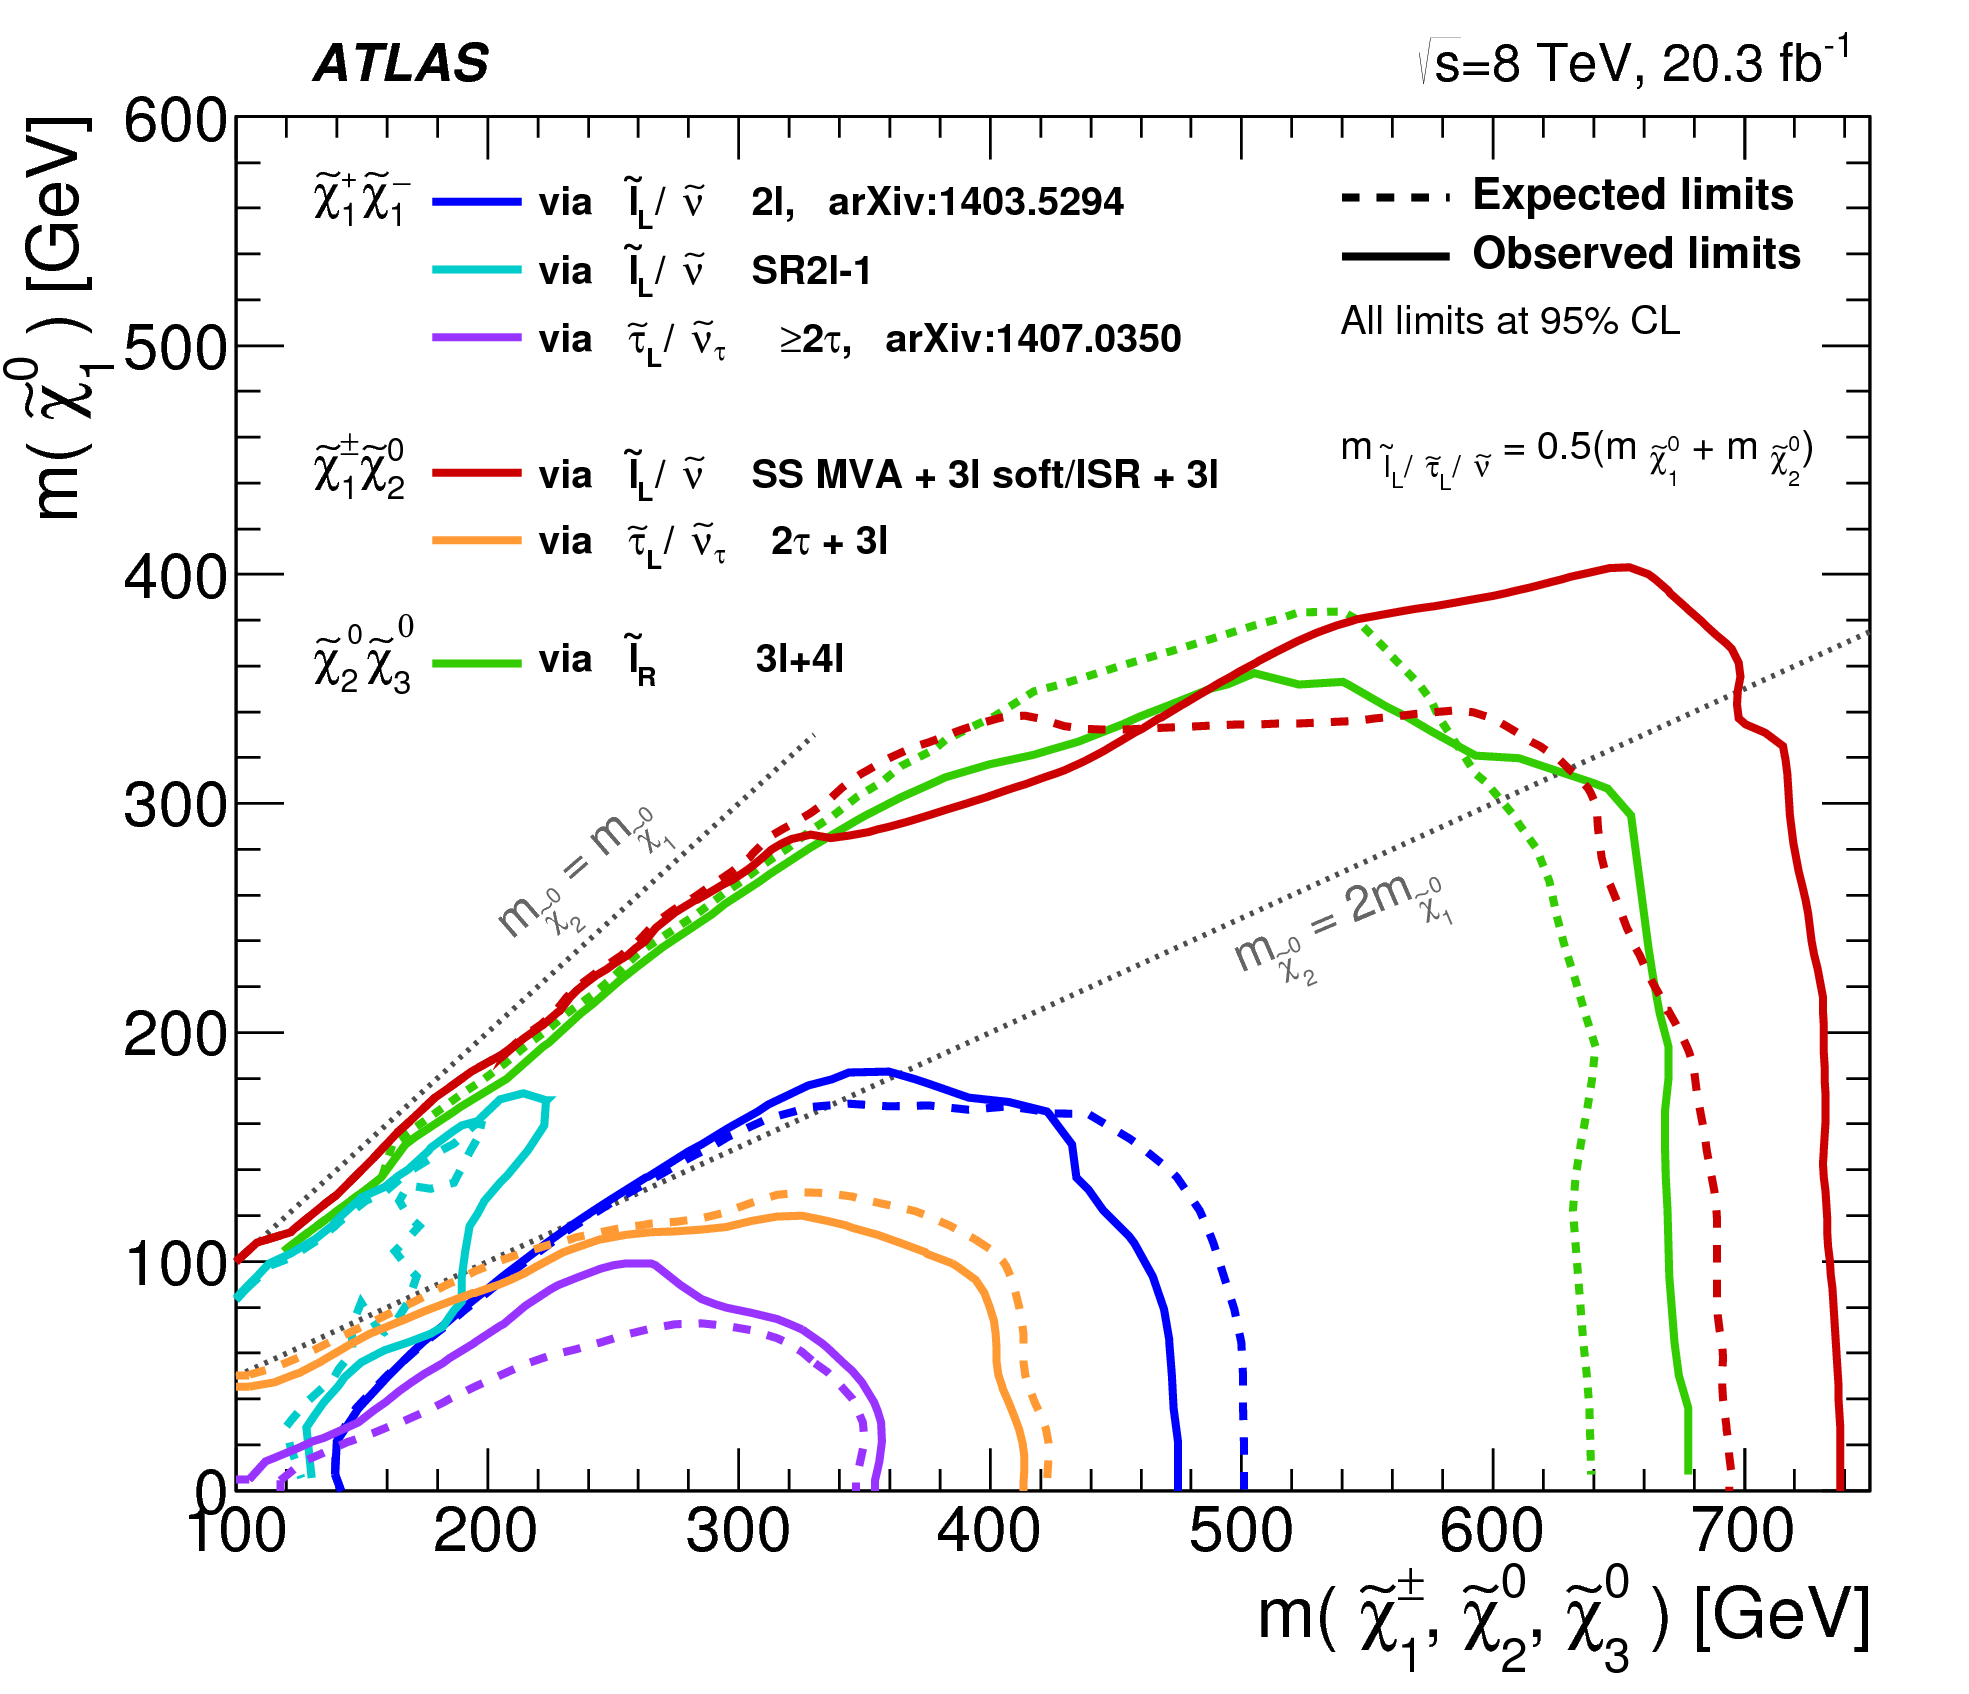
\includegraphics[scale=0.15]{Chap3/fig_19b}
	\caption{The 95\% CL exclusion limits on $\chi_1^+\chi_1^-$, $\chi_1^{\pm}\chi_2^0$ and $\chi_2^0\chi_3^0$ production with $l$-mediated decays, as a function of the $\chi_1^{\pm},\,\chi_2^0$ and $\chi_1^0$ masses \citep{aad2016search}. }\label{fig:summaryplot}
\end{figure}

These results are taken from \citep{atlas2015search} analysis performed at $\sqrt{s}=$8 TeV and integrated luminosity of 20.3 fb\textsuperscript{-1}. This search was performed based on various scenarios of the pMSSM, involving electroweak production of charginos and neutralinos. The turquoise and blue lines represent decay scenarios that are relevant for this paper as they show information on slepton-mediated decays of a chargino pair. 
In particular, the production of $\tilde{\chi}^{+}_{1}\tilde{\chi}^{-}_{1}$ pair decaying through a slepton ($\tilde{l}$) with final states contatining two opposite sign leptons will be considered (see Fig. \ref{fig:EWchargino}). 
\begin{figure}[!h]
  \centering   	
  	\captionsetup{width=0.8\textwidth}
	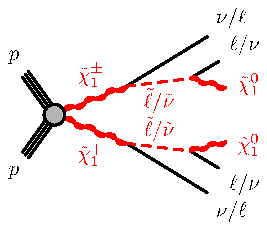
\includegraphics[]{Chap2/C1C1-llvvN1N1-slsnu}	
\caption[Optional caption for list of figures]{Electroweak chargino pair production in proton-proton collisions with intermediate slepton in the decay process.}\label{fig:EWchargino}
\end{figure}  

In the nomenclature used at LHC and in this thesis, electrons and muons are called "light leptons". Taus are considered separately as they decay very promptly and therefore are very difficult to reconstruct. This thesis only focuses on final states containing electrons and muons and the designation "lepton" only refers to these particles.  


%However, given that so far only 3.2 fb\textsuperscript{-1} of integrated luminosity has been achieved at $\sqrt{s} = 13$ TeV.

\subsection{Search methods}
Detecting new physics events at LHC requires using computational and statistical methods that can deal with the type of information a particle accelerator produces. The data is initially collected using triggers corresponding to the type of events under analysis. Each event has a large number of physical characteristics such as momentum, energy, mass, multiplicities, etc. The numbers representing them are all stored in a data structure which then can be accessed, modified and analysed using software tools. 

The cornerstone of all accelerator physics analyses is the correct estimation of background events. All background events represent physics that is already known and that has some similar or identical features with the processes we wish to study. For instance, this thesis focusses on the  reactions that have precisely two oppositely charged leptons in their final states. A number of processes well described by the standard model share this characteristic and therefore will form the background. 

The presence or absence of a new particle also can reveal itself in a number of ways. The case that is the easiest to detect is when there is an abnormality in mass distribution, such as the case with Higgs particle discovery. The peak in mass distribution of diphoton events constituted a significant excess over SM predictions \citep{chatrchyan2012observation,Aad:2012tfa}. 

This method does not work for SUSY particles and other techniques have to be used. Standard search techniques involve defining \textbf{signal regions} in data distributions that are sensitive to possible SUSY signals and looking whether there is a significant excess over SM background predictions in these regions. Another method is looking for abnormal tails in distributions that are not in agreement with SM predictions.   


%The overall goal is to have a procedure that loops over all events and selects those that are of interest for further analysis. 

 \chapter{Determining signal regions}
 \label{chap:results}
 %\section{Applying cuts to the same flavour channel}
\section{First view}

A common practice in SUSY dilepton analyses is to divide events into same flavour (SF) and different flavour (DF) varieties. SF thus includes events with pairs of only electrons or only muons in their final states, and DF refers to the events that decay into an electron-muon pair. In this analysis this convention will be followed.

The preliminary cuts on the pair of electrons were $\mathbf{p}_{\text{T},e_1}>$ 25 GeV and $\mathbf{p}_{\text{T},e_2}>$ 20 GeV, where $e_1$ refers to the leading lepton with the largest momentum and $e_2$ to the second one.  For a muon pair the following requirements were imposed: leading muon $\mathbf{p}_{\text{T},\mu_1}>$ 25 GeV, second muon $\mathbf{p}_{\text{T},\mu_2}>$ 10 GeV, and the invariant mass $m_{\mu \mu}>$ 20 GeV. These cuts were motivated by the trigger efficiency for offline lepton candidates' identification (see Fig. \ref{fig:eltrig} and \ref{fig:mutrig} in the appendix \ref{app:triggers}).

First, histograms showing the entirety of the 2015 data, MC background and signal simulations were plotted. Fig. \ref{fig:SF_total_mll} shows the distribution of the \dileptonmass \, in the SF channel. The largest background contributions come from the $Z$+jets, diboson, and $t\bar{t}$ processes. 
The pronounced peak in the SF dilepton invariant mass distribution is in the 80-100 GeV bin due to the contribution from the $Z$+jets component. This background can be suppressed by introducing $Z$ veto which cuts out all events within 10 GeV from the mass of the $Z$ boson (91.2 GeV). However, after this cut, the distribution will still retain events from the off mass-shell decays of the $Z$ boson. 

The histogram for DF channel (Fig. \ref{fig:DF_total_mll}) shows that there is a much smaller contribution from $Z$+jets component in this channel compared to the SF one. Thus $Z$ veto here can be avoided. The diboson and $t\bar{t}$ processes, however, prevail in this channel as well. 

\begin{figure}[!th]	   
	\begin{subfigure}[t]{0.5\textwidth}
		\subcaption{} 
		\label{fig:SF_total_mll}
        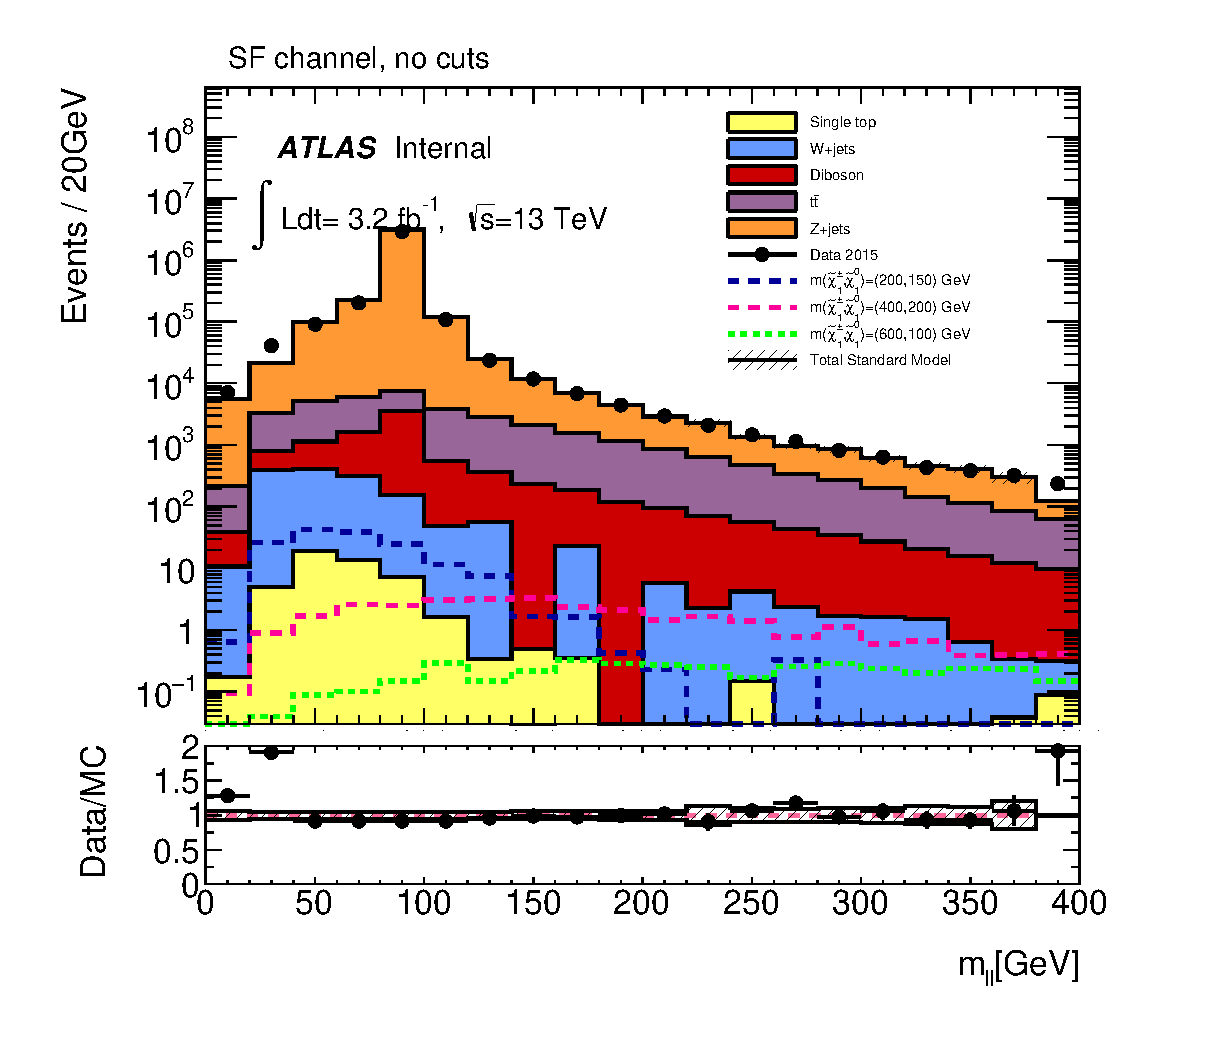
\includegraphics[scale=0.42]{Chap4/SF_DileptonMll_13TeV_total_signal} 
        \end{subfigure} 
     \begin{subfigure}[t]{0.5\textwidth}
     \subcaption{}
     	\label{fig:DF_total_mll}
        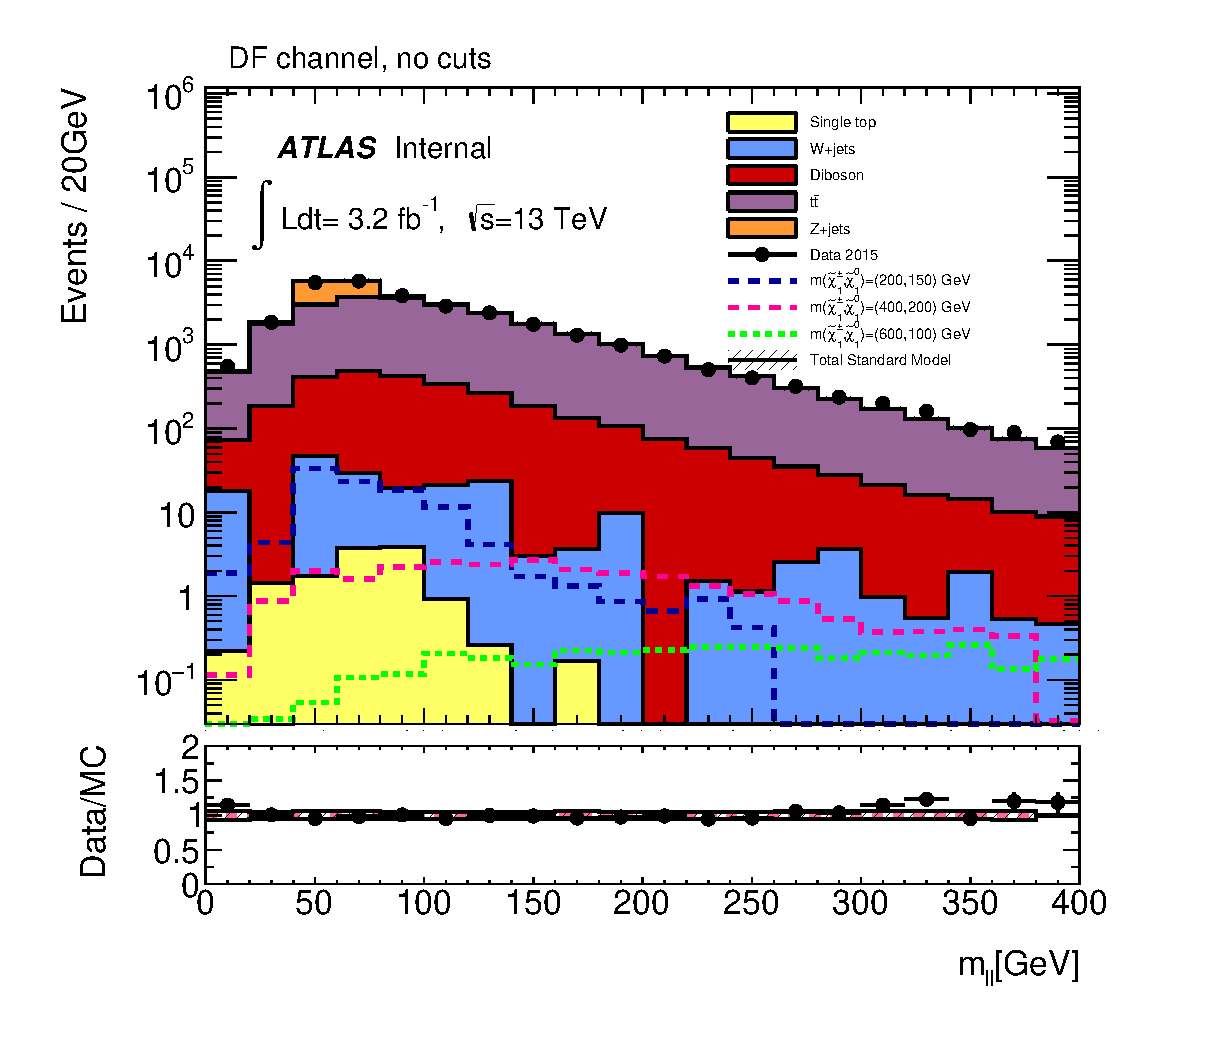
\includegraphics[scale=0.42]{Chap4/Emu_DileptonMll_13TeV_total_signal} 
        \end{subfigure}
        \begin{subfigure}[t]{0.5\textwidth}
		\subcaption{} 
		\label{fig:SF_total_mt2}
        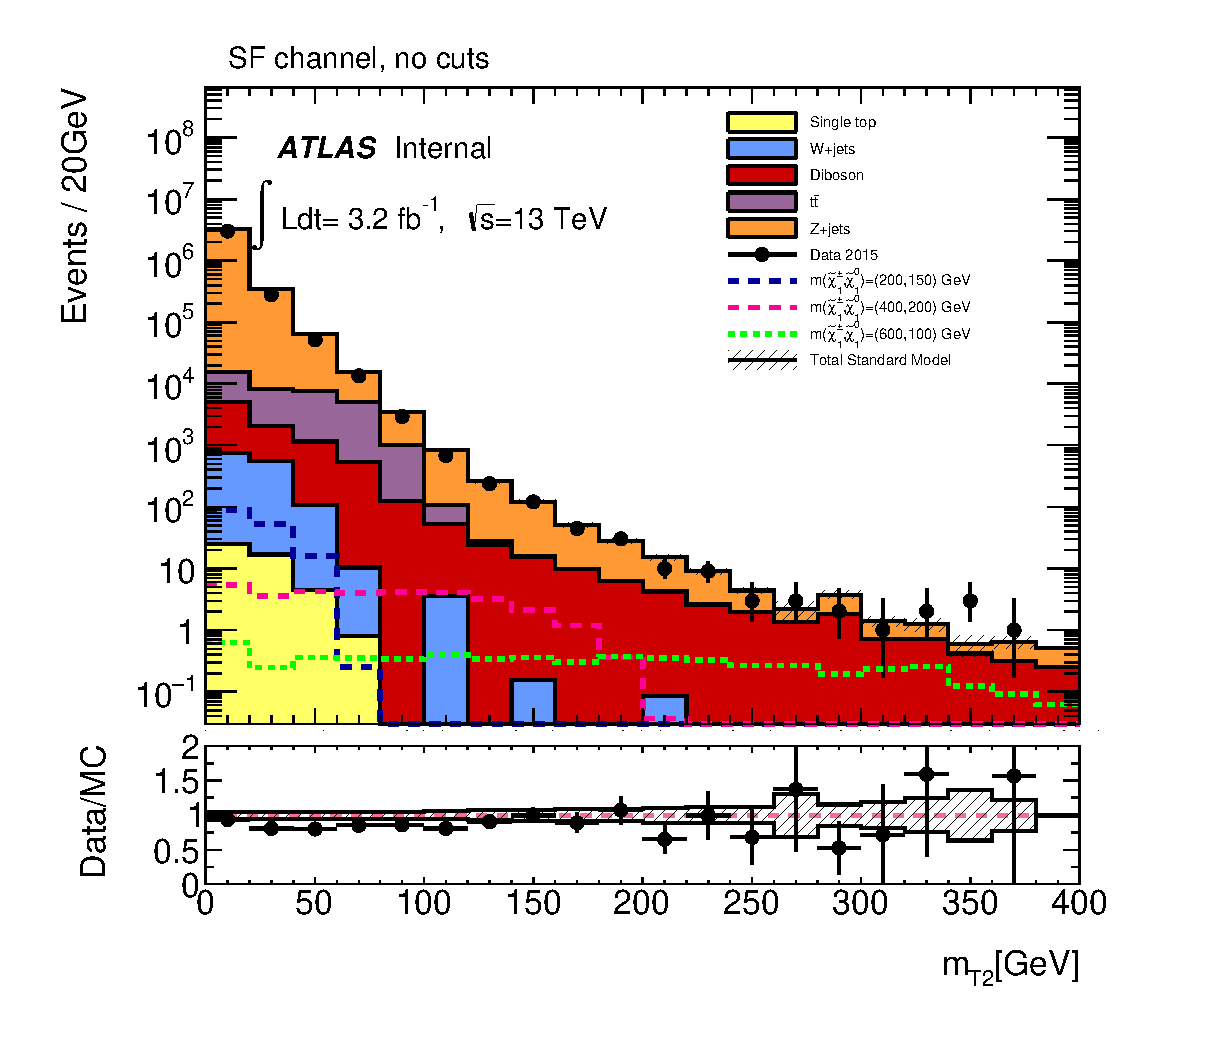
\includegraphics[scale=0.42]{Chap4/SF_DileptonMt2_13TeV_total_signal} 
        \end{subfigure} 
     \begin{subfigure}[t]{0.5\textwidth}
     \subcaption{}
     	\label{fig:DF_total_mt2}
        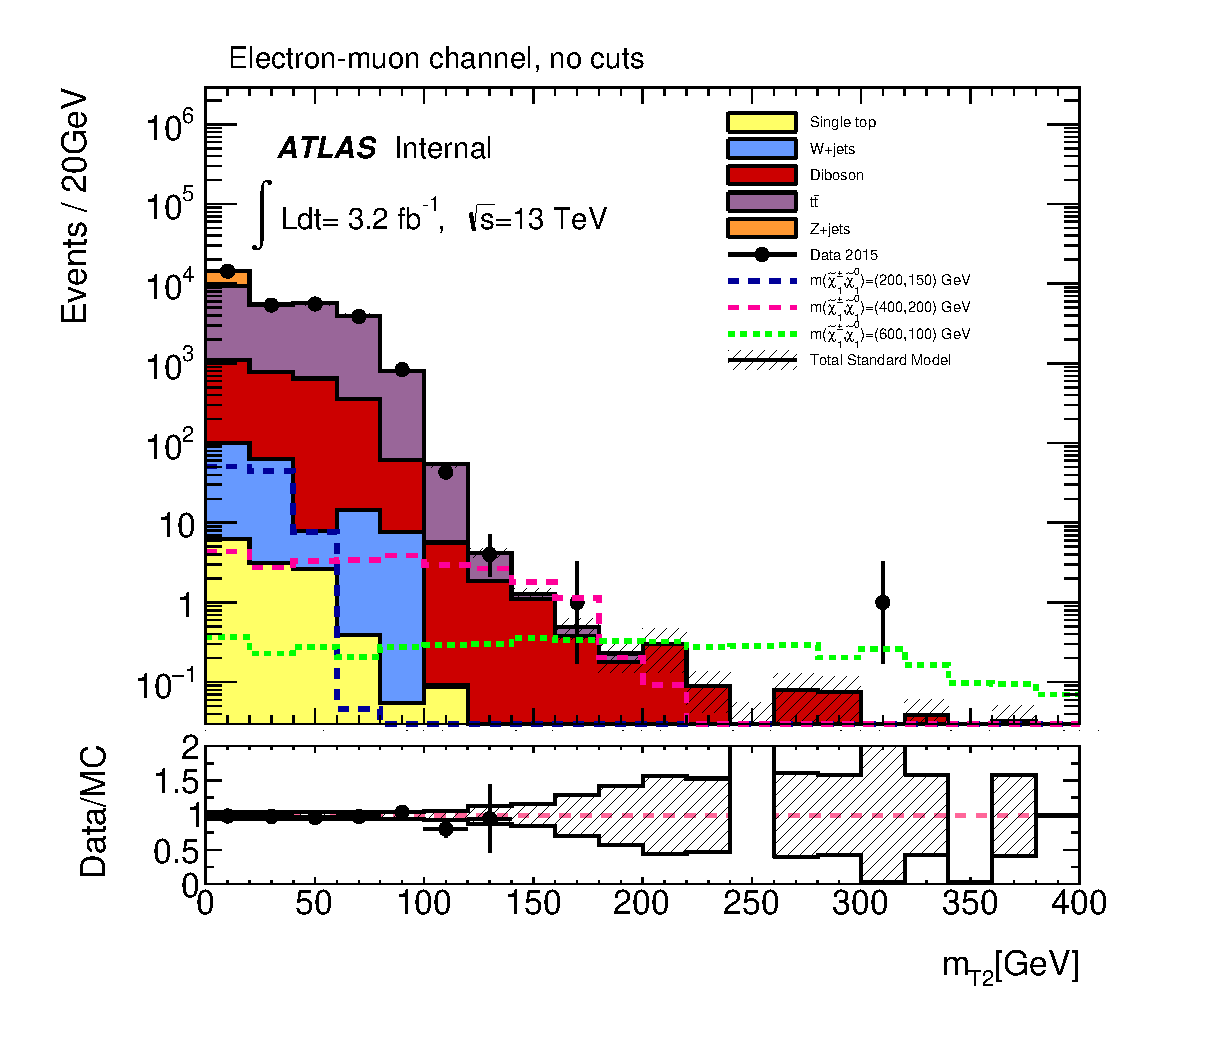
\includegraphics[scale=0.42]{Chap4/Emu_DileptonMt2_13TeV_total_signal} 
        \end{subfigure}
        \captionsetup{width=0.8\textwidth}
\caption{Distribution of $m_{\ell \ell}$ and \mttwo \, variables for SF and DF channels for all events.}	
        \label{fig:Elmu_total_histos}
\end{figure}

The dotted lines are the shapes of signal distributions and they are in accordance with the mass of the chargino pair. The blue line represents 200-150 mass splitting, so its events are concentrated in the lower mass regions. The pink and green lines represent 400-200 and 600-100 signals respectively, and also are distributed according to this logic. Overall, there is a good agreement between MC background simulations and the 2015 data. 

The total error of the background distribution, shown as hashed lines in the histograms, is calculated using simple poissonian statistics. Full error is a composite estimate that includes all sources of error and their interdependence, it entails a complex analysis that is beyond the scope of this thesis. 

\newpage
\section{Applying cuts}
\subsection{Veto on all jets.}

As was mentioned in the previous section the the following veto was imposed on all the signal regions in SF channel:
\begin{equation*}
|m_{\ell \ell} - m_Z| > 10 \text{ GeV (with } m_Z = 91.2 \text{ GeV}) 
\end{equation*}
This $Z$ veto is common for all further analyses in the SF channel, however it is not used at all for the DF channel.
The next step was to veto all the jets to reduce $t\bar{t}$ contribution. The result of this combination of vetoes can be seen in Fig. \ref{fig:0jets_mz}. As expected the \mttwo \, distribution is dependent on the mass splitting and is better for the 400-200 and 600-100 signals. At this point it is possible to calculate sensitivity values by placing cuts on \mttwo \, and the results can be seen in Tab. \ref{tab:SF_score}. No events from the 200-150 signal model passed the cuts, and therefore it is omitted from the table. The best result for the SF channel was the projected significance of 3.62 at 19.2 fb\textsuperscript{-1}  with \mttwo$>100$ GeV cut. The same cut for DF channel lead to the significance of 5.15  at \lumi =19.2 fb\textsuperscript{-1}. Significances for the 600-100 signal were not high in both channels, but were better for DF distributions, although not overwhelmingly so. 

\begin{figure}[h!]
\captionsetup{width=0.8\textwidth}	   
	\begin{subfigure}[t]{0.5\textwidth}
		\subcaption{$Z$ veto, no jets} 
		\label{fig:SF_0jets_mz_mt2}
        \includegraphics[scale=0.42]{Nojetsmz/SF_DileptonMt2_13TeV_0jets_mz_signal} 
        \end{subfigure} 
     \begin{subfigure}[t]{0.5\textwidth}
		\subcaption{No jets} 
		\label{fig:DF_0jets_mz_mt2}
        \includegraphics[scale=0.42]{Nojetsmz/Emu_DileptonMt2_13TeV_0jets_mz_signal} 
        \end{subfigure}      
\caption{The \mttwo \, distributions for SF and DF channels, with $Z$ veto (only for SF events) and no jets.}	
        \label{fig:0jets_mz}
\end{figure}
\begin{table}[H]
\centering
\captionsetup{width=0.8\textwidth}
\begin{tabular}{|l|llllll}
\hline
Signal models     & \multicolumn{1}{l|}{400-200} & \multicolumn{1}{l|}{600-100} & \multicolumn{1}{l|}{400-200} & \multicolumn{1}{l|}{600-100} & \multicolumn{1}{l|}{400-200} & \multicolumn{1}{l|}{600-100} \\ \hline
\hspace{5mm} \lumi     & \multicolumn{2}{c|}{3.2 \invfb}                                                     & \multicolumn{2}{c|}{9.6 \invfb}                                                     & \multicolumn{2}{c|}{19.2 \invfb}                                                    \\ \hline 
 \mttwo \, cut [GeV]            & \multicolumn{6}{c|}{\textbf{SF channel}}                                                                                                                                                                                                                   \\ \hline
$>80$  & \multicolumn{1}{l|}{1.01}               & \multicolumn{1}{l|}{0.26}               & \multicolumn{1}{l|}{1.74}               & \multicolumn{1}{l|}{0.45}               & \multicolumn{1}{l|}{2.46}               & \multicolumn{1}{l|}{0.64}               \\ \hline
$>100$ & \multicolumn{1}{l|}{1.47}               & \multicolumn{1}{l|}{0.50}               & \multicolumn{1}{l|}{2.56}               & \multicolumn{1}{l|}{0.86}               & \multicolumn{1}{l|}{3.62}               & \multicolumn{1}{l|}{1.22}               \\ \hline
$>120$  & \multicolumn{1}{l|}{1.27}               & \multicolumn{1}{l|}{0.61}               & \multicolumn{1}{l|}{2.19}               & \multicolumn{1}{l|}{1.06}               & \multicolumn{1}{l|}{3.09}               & \multicolumn{1}{l|}{1.5}                \\ \hline
                  & \multicolumn{6}{c|}{\textbf{DF channel}}                                                                                                                                                                                                                  \\ \hline
$>80$   & \multicolumn{1}{l|}{1.12}               & \multicolumn{1}{l|}{0.31}               & \multicolumn{1}{l|}{1.95}               & \multicolumn{1}{l|}{0.54}               & \multicolumn{1}{l|}{2.76}               & \multicolumn{1}{l|}{0.76}               \\ \hline
$>100$   & \multicolumn{1}{l|}{2.10}               & \multicolumn{1}{l|}{0.75}               & \multicolumn{1}{l|}{3.64}               & \multicolumn{1}{l|}{1.30}               & \multicolumn{1}{l|}{5.15}               & \multicolumn{1}{l|}{1.83}               \\ \hline
$>120$    & \multicolumn{1}{l|}{2.10}               & \multicolumn{1}{l|}{1.07}               & \multicolumn{1}{l|}{3.65}               & \multicolumn{1}{l|}{1.86}               & \multicolumn{1}{l|}{5.16}               & \multicolumn{1}{l|}{2.63}               \\ \hline
\end{tabular}
\caption{Significance values ($S/\sqrt{B}$) for the SF and DF channel signal models with various cuts on \mttwo \, at increasing integrated luminosities. Cuts include $Z$ veto (only for SF) and no jets are allowed.}
\label{tab:SF_score}
\end{table}


\subsection{Veto on $b$-tagged jets.}

Instead of vetoing all jets, a different cut vetoing only $b$-tagged jets was made and the resulting histograms can be seen in Fig. \ref{fig:SF_0bjets_mz}. The $b$-jet veto is evidently less drastic and leads to both more background and signal events in the final distribution. In order to see whether this cut makes difference compared to the no-jets cut, the significances have to be calculated. The resulting values can be seen in Table \ref{tab:SF_score_0bjets}. Again, no events from the 200-150 signal model passed the cuts and this model was omitted.

The $b$-jet veto leads to a decrease in significance for SF channel compared to the same cuts with no jets allowed. However, for DF channel significance values are higher. At \lumi= 19 \invfb \, and \mttwo $>120$ GeV, the 400-200 signal gives the significance of 6.77, and the 600-100 model has significance of 4.85 for  \mttwo$>140$ GeV. The difference in response of the SF and DF channels to the b-jet veto is due to the effect of the $Z$+jets background. It is more prevalent in the SF channel and therefore suppressed better by not allowing jets. 

 

\begin{figure}[H]	   
	\begin{subfigure}[t]{0.5\textwidth}
		\subcaption{$Z$ veto, no $b$-jets} 
		\label{fig:SF_0jets_mz_mt2}
        \includegraphics[scale=0.42]{Chap4/SF_DileptonMt2_13TeV_0bjets_mz_signal} 
        \end{subfigure} 
     \begin{subfigure}[t]{0.5\textwidth}
     \subcaption{No $b$-jets}
     	\label{fig:SF_0jets_mz_metrel}
        \includegraphics[scale=0.42]{Chap4/Emu_DileptonMt2_13TeV_0bjets_mz_signal} 
        \end{subfigure}
        \captionsetup{width=0.8\textwidth}
\caption{The \mttwo \, distributions for the SF and DF channels, with $Z$ veto and no $b$-jets.}	
        \label{fig:SF_0bjets_mz}
\end{figure}
\begin{table}[H]
\centering
\captionsetup{width=0.8\textwidth}
\begin{tabular}{|l|llllll}
\hline
Signal models     & \multicolumn{1}{l|}{400-200} & \multicolumn{1}{l|}{600-100} & \multicolumn{1}{l|}{400-200} & \multicolumn{1}{l|}{600-100} & \multicolumn{1}{l|}{400-200} & \multicolumn{1}{l|}{600-100} \\ \hline
\hspace{5mm} \lumi     & \multicolumn{2}{c|}{3.2 \invfb}                                                     & \multicolumn{2}{c|}{9.6 \invfb}                                                     & \multicolumn{2}{c|}{19.2 \invfb}                                                    \\ \hline 
 \mttwo \, cut [GeV]            & \multicolumn{6}{c|}{\textbf{SF channel}}                                                                                                                                                                                                                   \\ \hline
$>80$  & \multicolumn{1}{l|}{0.48}               & \multicolumn{1}{l|}{0.14}               & \multicolumn{1}{l|}{0.84}               & \multicolumn{1}{l|}{0.25}               & \multicolumn{1}{l|}{1.19}               & \multicolumn{1}{l|}{0.35}               \\ \hline
$>100$ & \multicolumn{1}{l|}{0.63}               & \multicolumn{1}{l|}{0.24}               & \multicolumn{1}{l|}{1.09}               & \multicolumn{1}{l|}{0.41}               & \multicolumn{1}{l|}{1.54}               & \multicolumn{1}{l|}{0.59}               \\ \hline
$>120$  & \multicolumn{1}{l|}{0.65}               & \multicolumn{1}{l|}{0.34}               & \multicolumn{1}{l|}{1.12}               & \multicolumn{1}{l|}{0.60}               & \multicolumn{1}{l|}{1.58}               & \multicolumn{1}{l|}{0.84}                \\ \hline
                  & \multicolumn{6}{c|}{\textbf{DF channel}}                                                                                                                                                                                                                  \\ \hline
$>80$   & \multicolumn{1}{l|}{0.94}               & \multicolumn{1}{l|}{0.29}               & \multicolumn{1}{l|}{1.64}               & \multicolumn{1}{l|}{0.50}               & \multicolumn{1}{l|}{1.49}               & \multicolumn{1}{l|}{0.45}               \\ \hline
$>100$   & \multicolumn{1}{l|}{2.06}               & \multicolumn{1}{l|}{0.85}               & \multicolumn{1}{l|}{3.57}               & \multicolumn{1}{l|}{1.47}               & \multicolumn{1}{l|}{5.05}               & \multicolumn{1}{l|}{2.08}               \\ \hline
$>120$    & \multicolumn{1}{l|}{2.76}               & \multicolumn{1}{l|}{1.59}               & \multicolumn{1}{l|}{4.79}               & \multicolumn{1}{l|}{2.75}               & \multicolumn{1}{l|}{6.77}               & \multicolumn{1}{l|}{3.88}               \\ \hline
$>140$    & \multicolumn{1}{l|}{2.07}               & \multicolumn{1}{l|}{1.98}               & \multicolumn{1}{l|}{3.59}               & \multicolumn{1}{l|}{3.43}               & \multicolumn{1}{l|}{5.08}               & \multicolumn{1}{l|}{4.85}               \\ \hline
\end{tabular}
\caption{Significance values for \mttwo \, distributions in the SF and DF channels with cuts on \mttwo \, at increasing integrated luminosities. With $Z$ veto (SF only) and no $b$-jets. }
\label{tab:SF_score_0bjets}
\end{table}
\newpage
\subsection{Cuts in the same-flavour channel}
Further analysis in the SF channel included the already mentioned $Z$ veto and the ``no jets" requirement. Different cuts were tried, including limiting jet multiplicity, imposing cuts on 
$\mathbf{p}^{\text{jet}}_{\text{T}}$, limiting $\mathbf{p}_{\text{T}}$ of the leading jet, etc. Ultimately, most probably due to the high amount of pileup, they were not very efficient. One cut that delivered the best significance values at \lumi= 19.2 \invfb \, was requiring \metrel$>$80 GeV and \mttwo$>$100 GeV (see Fig. \ref{fig:SF_metrel}). This yielded a significance of 4.05 for the 400-200 signal. Requiring \mttwo$>$120 GeV gave a significance of 1.50 for the 600-100 signal, the same result as obtained by imposing the \mttwo$>$120 cut without the \metrel \, cut (see Tab. \ref{tab:SF_score}). Tab. \ref{tab:SF_80} shows the significance values for these cuts.

\begin{figure}[H]
 	\centering
        \includegraphics[scale=0.5]{Chap4/SF_DileptonMt2_13TeV_0jets_mz_MetRel>80_signal} 
	\captionsetup{width=0.8\textwidth}
	\caption{The \mttwo \, distribution for the SF channel, with $Z$ veto,no jets and \metrel$>$80 GeV.}
     \label{fig:SF_metrel}
\end{figure}
\begin{table}[H]
\centering
\captionsetup{width=0.8\textwidth}
\begin{tabular}{|l|llllll}
\hline
Signal models     & \multicolumn{1}{l|}{400-200} & \multicolumn{1}{l|}{600-100} & \multicolumn{1}{l|}{400-200} & \multicolumn{1}{l|}{600-100} & \multicolumn{1}{l|}{400-200} & \multicolumn{1}{l|}{600-100} \\ \hline
\hspace{5mm} \lumi     & \multicolumn{2}{c|}{3.2 \invfb}                                                     & \multicolumn{2}{c|}{9.6 \invfb}                                                     & \multicolumn{2}{c|}{19.2 \invfb}                                                    \\ \hline 
 \mttwo \, cut [GeV]            & \multicolumn{6}{c|}{\textbf{SF channel}}                                                                                                                                                                                                                   \\ \hline
$>100$ & \multicolumn{1}{l|}{1.65}               & \multicolumn{1}{l|}{0.56}               & \multicolumn{1}{l|}{2.87}               & \multicolumn{1}{l|}{0.97}               & \multicolumn{1}{l|}{4.05}               & \multicolumn{1}{l|}{1.37}               \\ \hline
$>120$  & \multicolumn{1}{l|}{1.27}               & \multicolumn{1}{l|}{0.61}               & \multicolumn{1}{l|}{2.19}               & \multicolumn{1}{l|}{1.06}               & \multicolumn{1}{l|}{3.10}               & \multicolumn{1}{l|}{1.50}                \\ \hline               
\end{tabular}
\caption{Significance values for the SF channel with cut on \mttwo \, at increasing integrated luminosities. With $Z$ veto, no jets, and \metrel$>$80 GeV. }
\label{tab:SF_80}
\end{table}

Overall, significance in the SF channel was low for the two signals that passed the cuts. However, higher luminosities are likely to lead to better sensitivity values for both the 400-200 and 600-100 signal models. There are no significance values for the 200-150 model, although this model has the highest cross-section value. It is in the region which is overwhelmed with background and its suppression is very challenging. One way to deal with this will be discussed in the subsection \ref{subsec:200model}.

\subsection{Cuts in the different-flavour channel}

The electron-muon signal models overall provide better significance results, and good significance has already been obtained in the simple ``no $b$-jets" plus \mttwo \, cut (see Tab. \ref{tab:SF_score_0bjets}). However, further investigation was made to see if there is any improvement over those results.
For this channel the $Z$ veto does not apply and only $b$-jets are vetoed.

Higher values for sensitivity for the 400-200 and 600-100 signals were obtained with the following cuts - a)\metrel$>$40 GeV and \mttwo$>$120 GeV and b)\metrel$>$80 GeV and \mttwo$>$120 GeV. The resulting histograms are in Fig. \ref{fig:DF_mt2} and the sensitivities can be seen in the accompanying Table \ref{tab:DF_significances}.

\begin{figure}[h!]
\captionsetup{width=0.8\textwidth}	   
	\begin{subfigure}[t]{0.5\textwidth}
		\subcaption{No $b$-jets, \metrel$>$40 GeV} 
		\label{fig:DF_mt2_metrel40}
        \includegraphics[scale=0.42]{Chap4/Emu_DileptonMt2_13TeV_0bjets_mz_MetRel>40_signal} 
        \end{subfigure} 
     \begin{subfigure}[t]{0.5\textwidth}
		\subcaption{No $b$-jets, \metrel$>$80 GeV} 
		\label{fig:DF_mt2_metrel80}
        \includegraphics[scale=0.42]{Chap4/Emu_DileptonMt2_13TeV_0bjets_mz_MetRel>80_signal} 
        \end{subfigure}      
\caption{The \mttwo \, distributions for the DF channel with $b$-jet veto and different cuts on \metrel.}	
        \label{fig:DF_mt2}
\end{figure}
\begin{table}[H]
\centering
\captionsetup{width=0.8\textwidth}
\begin{tabular}{|l|llllll}
\hline
Signal models     & \multicolumn{1}{l|}{400-200} & \multicolumn{1}{l|}{600-100} & \multicolumn{1}{l|}{400-200} & \multicolumn{1}{l|}{600-100} & \multicolumn{1}{l|}{400-200} & \multicolumn{1}{l|}{600-100} \\ \hline
\hspace{5mm} \lumi     & \multicolumn{2}{c|}{3.2 \invfb}                                                     & \multicolumn{2}{c|}{9.6 \invfb}                                                     & \multicolumn{2}{c|}{19.2 \invfb}                                                    \\ \hline 
 Cuts            & \multicolumn{6}{c|}{\textbf{DF channel}}                                                                                                                                                                                                                   \\ \hline
\footnotesize{\metrel$>$40 GeV, \mttwo$>$120 GeV} & \multicolumn{1}{l|}{2.78}               & \multicolumn{1}{l|}{1.59}               & \multicolumn{1}{l|}{4.81}               & \multicolumn{1}{l|}{2.76}               & \multicolumn{1}{l|}{6.80}               & \multicolumn{1}{l|}{3.90}               \\ \hline
\footnotesize{\metrel$>$80 GeV, \mttwo$>$120 GeV} & \multicolumn{1}{l|}{2.80}               & \multicolumn{1}{l|}{1.61}               & \multicolumn{1}{l|}{4.85}               & \multicolumn{1}{l|}{2.78}               & \multicolumn{1}{l|}{6.86}               & \multicolumn{1}{l|}{3.93}                \\ \hline               
\end{tabular}
\caption{DF channel significances with cuts on \mttwo \, and \metrel \, at increasing integrated luminosities. $b$-jets are vetoed.}
\label{tab:DF_significances}
\end{table}

The DF channel provides better sensitivity that the SF channel with relatively few cuts. So if the evidence of SUSY lies in this channel it should be relatively easy to confirm. However, this also requires higher luminosity. The 200-150 model does not produce any significance in this channel as well, again due to being in a background-dominated region. The next subsection offers one way this issue can be addressed.

\subsection{Further investigation of the 200-150 signal}
\label{subsec:200model}

So far, the 200-150 signal proved to be hard to discern from the background. However, there is a method that can potentially yield some sensitivity for this model. It is based on the assumption that the chargino pair creation recoils against a single leading jet which gives additional momentum to the neutralinos in the final state \citep{atlas2015search}. Thus the angle $\Delta\phi(E^{\text{miss}}_{\text{T}},\text{jet})$ between \met \, and the leading jet can be exploited as a discriminating variable. The histograms in Figure \ref{fig:DF_dPhi} show this relation for the DF channel. 

\begin{figure}[th!]
\captionsetup{width=0.8\textwidth}	   
	\begin{subfigure}[t]{0.5\textwidth}
		\subcaption{One jet, \met$>$80 GeV} 
		\label{fig:DF_dPhi80}
        \includegraphics[scale=0.4]{Chap4/Emu_OneCentralJet_dPhiMetJet_13_TeV_signal_80} 
        \end{subfigure} 
     \begin{subfigure}[t]{0.5\textwidth}
		\subcaption{One jet, \met$>$100 GeV} 
		\label{fig:DF_dPhi100}
        \includegraphics[scale=0.4]{Chap4/Emu_OneCentralJet_dPhiMetJet_13_TeV_signal_100} 
        \end{subfigure}      
\caption{The $\Delta\phi(E^{\text{miss}}_{\text{T}},\text{jet})$ distributions for the DF channel with single jet, \dileptonmass$>$40 GeV and cuts on \met.}	
        \label{fig:DF_dPhi}
\end{figure}

\begin{table}[!H]
\centering
\captionsetup{width=0.8\textwidth}
\begin{tabular}{|l|l|l|l|}
\hline
    Signal    & \multicolumn{3}{c|}{200-150}       \\ \hline
\hspace{5mm}\lumi   & 3.2\invfb & 9.6\invfb & 19.2\invfb \\ \hline
\met$>$80 GeV,$\Delta\phi(E^{\text{miss}}_{\text{T}},\text{jet})>2.7$ & 0.60      & 1.04      & 1.47       \\ \hline
\met$>$100 GeV,$\Delta\phi(E^{\text{miss}}_{\text{T}},\text{jet})>2.9$    & 0.40      & 0.70      & 0.99       \\ \hline
\end{tabular}
\caption{Significances for the $\Delta\phi(E^{\text{miss}}_{\text{T}},\text{jet})$ distributions for the DF channel with single jet. }
\label{tab:DF_jet}
\end{table}

The 200-150 signal is concentrated at large values for $\Delta\phi(E^{\text{miss}}_{\text{T}},\text{jet})$ and thereby in agreement with the recoil assumption. However, in these regions the significance values are not high, as can be seen in the Table \ref{tab:DF_jet}.
 
The best significance value for this search method was 1.47 at 19.2 \invfb \, for the \met$>$80 GeV,$\Delta\phi(E^{\text{miss}}_{\text{T}},\text{jet})>2.7$ combined cut. It is still quite small and does not satisfy statistical criteria for good sensitivity. However, there is a clear dependence of a smaller mass signal on the recoil angle with the leading jet. This can be a starting point for other analyses that can take into account other variables as well. 












\startappendices
\appendix{Trigger Efficiencies}
\label{app:triggers}
\begin{figure}[h]
     \centering
        \captionsetup{width=0.7\textwidth}
        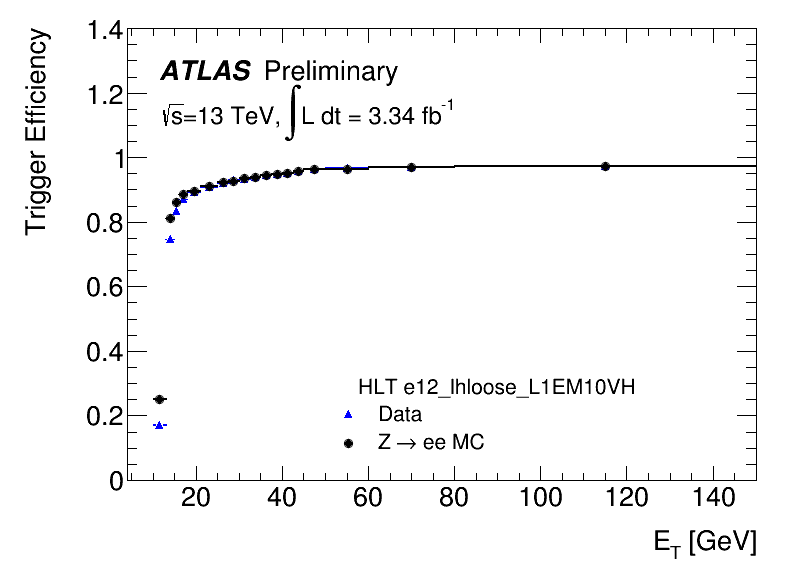
\includegraphics[width=8cm]{Appendices/Et_e12_lhloose_L1EM10VH}
        \caption{Electron trigger efficiency as a function of the off-line electron candidate’s $\mathbf{E_T}$ \citep{eltrig}.}
        \label{fig:eltrig}
\end{figure}%
\begin{figure}[h]
     \centering
        \captionsetup{width=0.7\textwidth}
        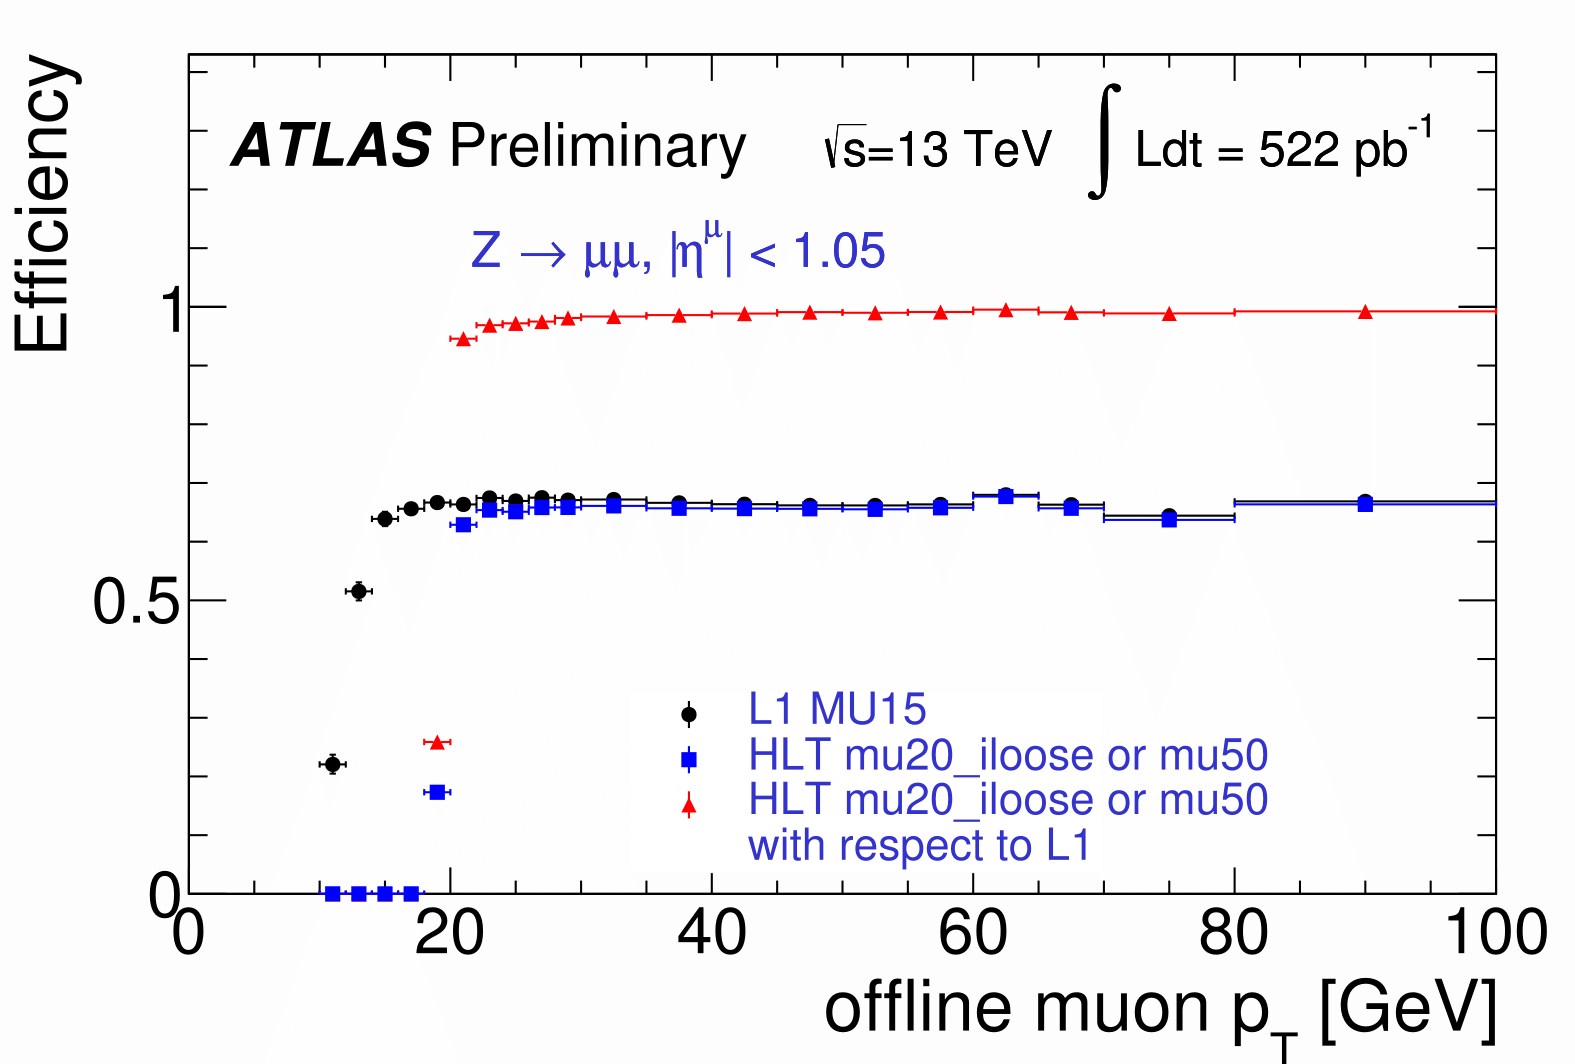
\includegraphics[width=8cm]{Appendices/LHCC_HLT_mu20_iloose_L1MU15_OR_HLT_mu50_barrel_probe_pt_eff}
        \caption{Muon trigger efficiency as a function of $\mathbf{p_T}$ of offline muon candidates \citep{muontrig}.}  
        \label{fig:mutrig}   
\end{figure}

%\appendix{Exclusion limits of ATLAS SUSY searches}
 %\label{app:SUSYlimit}
 %\begin{figure}[!ht]
\includegraphics[scale=0.17]{Appendices/ATLAS_SUSY_Summary.png}
\caption{Exclusion limits of ATLAS searches for Supersymmetry \citep{SUSYlimits}}
\label{fig:SUSYlimit}
\end{figure}
 
%\startbibliography
 \begin{singlespace} % Bibliography must be single spaced
  \bibliography{References}   % Use the BibTeX file ``References.bib''.
 \end{singlespace}

% An external Abstract that can be printed at the end of the document, 
% for separate submission to Rackham. Comment it out when not needed. - jg
%\startextabstractpage
%{The Title of Your Dissertation}{Your Name}{Chair: Albert Einstein}
%

%\label{ExtAbstract}

\end{document}
